\documentclass[t,slidestop,compress,mathserif,color=option,hyperref={pdfstartview={Fit},pdfpagelayout={SinglePage},pdfpagemode={UseOutlines}}]{beamer}

%\usepackage[envcountsect]{beamerarticle}

\usepackage{general-beamer}

\usetheme{Madrid}
\usecolortheme{seahorse}

%\usepackage{beamercolorthemeCalPoly}
%\usepackage{beamerinnerthemeCalPoly}
%\usepackage{beamerouterthemeCalPoly}
%\usepackage{beamerthemeCalPoly}

\usepackage{tikz}

\hypersetup{
  pdfstartview={Fit}
  pdfpagelayout={SinglePage}
  pdfpagemode={UseOutlines}
}

\xdefinecolor{blue}{rgb}{0.0,0.2,0.8}
\newcommand{\blue}[1]{{\color{blue}#1}}
\newcommand{\emblue}[1]{\emph{\color{blue}#1}}
\xdefinecolor{purple}{rgb}{0.4,0.0,0.6}
\newcommand{\purple}[1]{{\color{purple}#1}}
\xdefinecolor{red}{rgb}{0.8,0,0.2}
\newcommand{\red}[1]{{\color{red}#1}}
\xdefinecolor{green}{rgb}{0.2,0.6,0.2}
\newcommand{\green}[1]{{\color{green}#1}}
\newcommand{\CPgreen}[1]{{\color{CPgreen}#1}}

\newcommand*\diff{\mathop{}\!\mathrm{d}} % command for differential operator
\newcommand{\integral}[4][x]{\ensuremath{\displaystyle \int_{#3}^{#4} #2 \diff #1}}

\begin{document}

\allowdisplaybreaks

\title[Quaternions]
    {Quaternions 
        \begin{align*}
            \left\{t+xi+yj+zk: 
            \begin{aligned}
                & t, x, y, z \in \bR, \\
                & i^2 = j^2 = -1, \\
                & ij = -ji = k 
            \end{aligned}
            \right\}
        \end{align*}     
    }
\author[Andy, Bailey, Ian]
    {Andy Haase, Bailey Wickham, Ian Gallagher \\ Dr. Brussel}

\begin{frame}
  \titlepage
\end{frame}

\section{3D/4D Number System}
\subsection{Short Hamilton History?}

\begin{frame}{Hamilton}
    \begin{itemize}
        \item \bR is a 1D number system, \bC forms a 2D number system.
            Hamilton tried for years to create a 3D system. In the end, he created a 4D number system we now call the quaternions (\bH)
        \item Think of \bH as a 4D vector space over \bR. Hamilton discovered that there is a natural multiplication on this space, giving it the structure of a number system. 
        % We can mention that this doesn't always happen over other euc spaces out loud. 
    \end{itemize}
    \begin{figure}
        \centering
        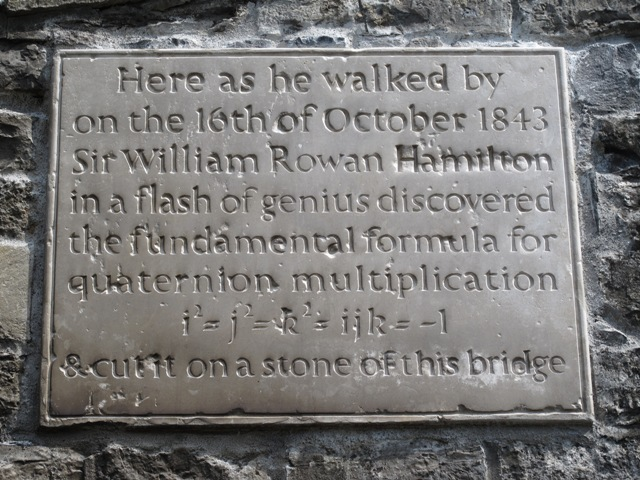
\includegraphics[c, scale=0.5]{H Pres/hamiltonbridge.jpg}
        \caption{Quaternions Plaque}
        \label{fig:hbridge}
    \end{figure}
\end{frame}

\subsection{Structure}

\begin{frame}{Multiplication Basics}
    %Put a basic description of H h
    \begin{center}
        $\bH = \left\{t + xi + yj + zk : t, x, y, z \in \bR, i^2=j^2=ijk=-1 \right\}$
    \end{center}
    \begin{center}
    	\begin{tikzpicture}[-latex, auto, node distance = 4cm and 5cm, on grid, semithick, state/.style = {circle, top color=white, draw, minimum width = 1cm}, scale=0.75]
            \node[state] at (2,3) (I) {$i$};	
            \node[state] at (4,0) (J) {$j$};	
            \node[state] at (0,0) (K) {$k$};	
    	
    	    \path (I) edge [bend left = 25] (J);
    	    \path (J) edge [bend left = 25] (K);
    	    \path (K) edge [bend left = 25] (I);
        \end{tikzpicture}
    \end{center}
    \begin{examples}
        \begin{align*}
            (3i-5j)(4j-k) &= 12ij - 3ik - 20j^2 + 5jk \\
                          &= 12k - 3(-j) - 20(-1) + 5i \\
                          &= 20 + 5i + 3j + 12k
        \end{align*}
    \end{examples}
\end{frame}

\begin{frame}{The 3-Sphere}
    \begin{itemize}
        \item $S^3$ is the set of points at distance 1 from the origin in \bH, which forms a "3-sphere" in 4D space, analogous to the usual 2-sphere in 3D space. 
        \item We can also show that $S^3$ is closed under multiplication in \bH, and therefore forms a {\it group}. It is one of the most important groups in mathematics and physics.
    \end{itemize}
    \begin{block}{Definition of $S^3$}
        \begin{center}
            %$\| t + xi + yj + zk \| = \sqrt{t^2 + x^2 + y^2 + z^2}$
            $S^3=\{(t,x,y,z)\in\bR^4:t^2+x^2+y^2+z^2=1\}.$
        \end{center}
    \end{block}
    
\end{frame}

%\begin{frame}{Conjugacy Classes of $S^3$}
%    \itemize
%    \item We are interested in Conjugacy Classes of elements in $S^3$, or elements that are "closely related". 
%    \begin{block}{Conjugacy Classes}
%    Elements $a$ and $b$ are conjugate if there exists $c$ such that $b = cac^{-1}$. The set of all elements conjugate to $a$ is called the "conjugacy class" of $a$
%    \end{block}
%   \item We showed that the conjugacy class for a given quaternion $a \in \mathbb{H}$ consists of all quaternions $b \in \mathbb{H}$ such that the real component of $a$ and $b$ are equal and the "imaginary" components of $a$ and $b$ are of equal length.
%    \begin{block}{Imaginary Components and Pure Imaginary Elements}
%        The imaginary component of a given element $a \in \mathbb{H}$ is the $xi+yj+zk$ component. For example, the imaginary component of $1+i+j+2k$ is $i+j+2k$. A pure imaginary element has no real part, so the imaginary component is entire quaternion.
%    \end{block}
%\end{frame}
%

\begin{frame}{Embeddings of \bC}
    \begin{itemize}
        \item Imagine all of the planes passing through the $x$-axis in 3D space. 
        \item This can be described as a ``circle of planes'' which, taken together, fill the space
        \item Extending this analogy to 4D space, we find there is a {\it sphere} of planes containing the $t$-axis
        \item These planes, we discovered, are each actually complex planes in disguise!
        \item $S^3$ acts transitively on these planes
    \end{itemize}
    
    \begin{block}{Square Roots of $-1$}
    \begin{center}
        $\left\{ xi + yj + zk \in \bH : x^2 + y^2 + z^2 = 1 \right\}$
    \end{center}
    \end{block}
\end{frame}

\begin{frame}{$2 \times 2$ Matrices and Their Planes}
\begin{itemize}
    \item \bH is a Central Simple Algebra (CSA). There is one other 4D CSA over \bR: the usual matrix ring $M_2(\bR)$. We sought to extend our idea of embedded planes to $M_2(\bR)$. 
    \item We found that there exist complex planes inside of $M_2(\bR)$, but unlike in \bH, the union of these planes is \alert{not} the entire ring.
    \item There are also two other types planes inside of $M_2(\bR)$, where the multiplication is not complex multiplication, but something different. The types are \bC, $\bR \times \bR$, and a 'degenerate' case, we call a {\it nilpotent plane}.
    \item An analog to $S^3$ acts transitively on each set of planes in $M_2(\bR)$
    % Multiplication in the degenerate plane $(a,b)*(c,d) = (ad + bc, bd)$ <------This is some bs right here
\end{itemize}
%\begin{figure}
%    \centering
%    \includegraphics[scale=.5\pagewidth]{H Pres/smileysphere3.jpg}
%    \caption{Amiable 2-Sphere}
%    \label{fig:smileysphere}
%\end{figure}
\end{frame}

\end{document}